Per attuare questo confronto tra mezzi di trasporto si è scelto di appoggiarsi a servizi di navigazione in grado di fornire stime di percorrenza in tempo reale per usarle come valori effettivi su cui basare le analisi. Le gare sono state tradotte in richieste per un tragitto comune, effettuate più volte al giorno e per diversi percorsi al fine di rendere possibile uno studio su degli stessi viaggi iniziati nello stesso istante. Sono stati presi in considerazione l'automobile e i principali mezzi di trasporto alternativi con cui è possibile spostarsi all'interno del Comune di Milano:
\begin{itemize}
	\item automobile;
	\item servizio di car sharing Enjoy;
	\item mezzi pubblici ATM e passanti ferroviari Trenord;
	\item bicicletta;
	\item a piedi.
\end{itemize}
Sebbene il servizio di car sharing riguardi comunque l'utilizzo di un'automobile, è stato preso in considerazione come mezzo alternativo per spostamenti occasionali. Questo servizio infatti permette di sfruttare molti dei vantaggi dell'auto senza possederne una e solo quando strettamente necessario, vantaggi validi fintanto che il costo dell'uso occasionale risulta più economico dell'acquisto e del mantenimento di un'auto privata. L'utilizzo di questo servizio in determinate condizioni riuscirebbe ad abbattere, oltre il costo dell'auto, il problema dell'inquinamento dovuto dal parco auto non aggiornato. La maggior parte delle aziende nel settore infatti offre una flotta molto aggiornata, a partire dalle Fiat 500 con standard Euro V per Enjoy\footnote{\url{https://enjoy.eni.com/it/milano/flotta}. Accessed: 20/01/2021} fino alle Smart Fortwo con motori Euro VI di ShareNow\footnote{\url{https://www.share-now.com/it/it/fleet/}. Accessed: 20/01/2021} (ex Car2Go). Il percorso a piedi, seppur non diretto competitore, è stato scelto per essere usato come riferimento.

\section{Ricerca delle API}

Il primo passo per la realizzazione di questo studio è stato quello di cercare delle Application Programming Interface (API) disponibili per ogni mezzo di trasporto in grado di fornire stime dinamiche sui tempi di percorrenza basate su dati in tempo reale.

\subsection{Google}

Inevitabilmente Google è stata la prima opzione che si è cercata, in grado di offrire stime di percorrenza per auto, bici, mezzi pubblici e percorsi a piedi. Google infatti, grazie a Maps e grazie all'acquisizione di Waze, è una dei leader nel settore delle informazioni di navigazione che vende la propria conoscenza e potenza di calcolo tramite API. Tra le varie opzioni in vendita al momento della ricerca era presente la Directions API\footnote{\url{https://developers.google.com/maps/documentation}. Accessed: 20/01/2021}, in grado di fornire stime di percorrenza molto precise per l'auto, per il percorso a piedi e per la bicicletta, quest'ultima solo in presenza di piste ciclabili lungo il percorso. Questa opzione è stata subito scartata per via del costo eccessivo del servizio di 10\$ per 1000 richieste al mese\footnote{\url{https://cloud.google.com/maps-platform/pricing/sheet}. Accessed: 20/01/2021}, l'equivalente di circa 1 richiesta all'ora, troppo poco per l'obiettivo dello studio di catturare la variazione oraria delle performance dei mezzi e troppo costoso per essere portato sulla scala voluta di almeno 10 richieste l'ora, una ogni dieci minuti.

\subsection{Waze}

Nonostante sia stata acquisita da Google, Waze è rimasta indipendente. È specializzata nelle stime di percorrenza in automobile e in moto. Quello che offre Waze però non sono esattamente delle API a cui fare richiesta per un determinato viaggio, ma semplicemente degli URL da inserire nel proprio sito web o nella propria applicazione Android/iOS per aprire il client Waze coi dati della richiesta parametrizzati nell'URL\footnote{\url{https://www.waze.com/sdk}. Accessed: 20/01/2021}.

\subsection{Moovit}

Anche Moovit, specializzata nei mezzi pubblici e nei treni, non offre API per interrogare direttamente i loro servizi e ricevere delle stime, ma solamente l'opzione di incorporare un widget all'iterno della propria pagina web o applicazione che rimanda direttamente ai loro servizi\footnote{\url{https://moovit.com/developers/}. Accessed: 20/01/2021}. Al momento della ricerca, Moovit offriva un servizio gratuito di API chiamato DeepLink la cui pagina risultava inaccessibile, restituendo il codice di stato HTTP 500, "Internal Server Error".

\subsection{Here}

Il servizio Here, specializzato nei percorsi in auto, scooter e mezzi pubblici, offre una REST API per le informazioni riguardo il routing e la stima del tempo di percorrenza\footnote{\url{https://developer.here.com/documentation}. Accessed: 20/01/2021}. Queste stime però risultano accurate, ovvero basate su dati in tempo reale, solo per determinate città comunicate sul loro sito, e tra queste non era inclusa Milano. Per le città non in lista, la stima è fatta staticamente sulla base di dati geografici o dei dati tabellari degli orari dei passaggi dei mezzi nel caso dei trasporti pubblici.

\subsection{Car2Go, Enjoy}

Non sono stati trovati servizi in grado di fornire stime di tempi di percorrenza utilizzando un mezzo dei servizi car sharing. I servizi Car2Go ed Enjoy non offrono API per tale calcolo ma dispongono di una mappa costantemente aggiornata sul loro sito web con l'elenco delle auto libere, ognuna con allegato dati riguardo il tipo di veicolo, tra auto e moto, e il carburante rimasto. Un software in grado di acquisire le informazioni delle auto libere è stato gentilmente offerto da Losacco Federico, che lo ha scritto e utilizzato per uno studio sul comportamento del traffico basato sui viaggi compiuti dagli utenti del servizio \cite{trentini2017sampling}.

\subsection{OpenStreetMap}

Il progetto collaborativo di OpenStreetMap offre, tra le altre cose, il calcolo di un tragitto usando come backend servizi offerti da terze parti, tra cui Open Source Routing Machine (OSRM), per stimare percorsi in auto, in bici e a piedi. Purtroppo però, tali servizi non usano dati in tempo reale \footnote{\url{https://wiki.openstreetmap.org/wiki/Routing}. Accessed: 20/01/2021}.

\section{Scelta delle API}

Di seguito sono elencate le scelte fatte per i servizi e i loro rispettivi ruoli di copertura dei mezzi di trasporto:

\begin{itemize}
	\item Here API
	\begin{itemize}
		\item mezzi pubblici ATM e passanti ferroviari Trenord;
	\end{itemize}

	\item OpenStreetMap con OSRM
	\begin{itemize}
		\item bicicletta e a piedi;
	\end{itemize}

	\item scraping di Enjoy Map usando il software di Losacco Federico \cite{trentini2017sampling}
	\begin{itemize}
		\item servizio di car sharing Enjoy;
	\end{itemize}

	\item scraping di Waze personalmente programmato
	\begin{itemize}
		\item mezzi pubblici ATM e passanti ferroviari Trenord;
	\end{itemize}
\end{itemize}
Nonostante OSRM non offra soluzioni in tempo reale è stato scelto ugualmente per via della scarsa influenza del traffico sui tempi di pecorrenza in bicicletta e a piedi, che dipendono per la maggior parte dall'itinerario calcolato e dalle caratteristiche delle strade, come segnali stradali di divieti, contromano e di aree pedonali. Le API di Here sono state utilizzate per mancanza di valide alternative. In un primo momento si è tentato lo scraping del sito web di Moovit per interagire col sito e comunicare le richieste senza intervento umano, ma la difficoltà nel codificare i parametri delle richieste e a decodificarne le poche risposte immerse in svariati messaggi di errore ne hanno scoraggiato l'utilizzo. Nella tabella \ref{table:1} sono stati riportati in percentuale gli errori dovuti all'impiego di Moovit. Per il servizio di car sharing si è scelto di usare la lista delle macchine libere come base, ottenuta tramite scraping, per ottenere una stima del tempo di percorrenza basata su due percorsi, per primo il tragitto a piedi per raggiungere l'auto libera più vicina al punto di partenza richiesto e come secondo il tragitto in auto per completare il percorso dal punto in cui si trova l'auto selezionata alla destinazione richiesta. Non sono state trovate valide alternative per il servizio di routing in automobile. Google risulta essere eccessivamente costosa se si considera un minimo di 10 richieste all'ora per avere un campione rappresentativo di un giorno da diversi punti della città. Il prezzo per una prestazione del genere è di circa 72\$ al mese. Waze invece non offre nessuna API per essere interrogata direttamente. Per ovviare a questo problema, si è scelto di programmare un browser headless in grado di interagire direttamente col sito web di Waze per interrogare il servizio e prelevare i dati della stima di percorrenza, simulando per intero l'interazione umana con la pagina. Le API di Here e quelle di OpenStreetMap invece chiedono in input le coordinate di partenza e di destinazione e restituiscono in output una stima di percorrenza del tragitto in formato JSON di quel determinato momento, oltre ad altri dati relativi alla tratta consigliata.

\subsection{Lo scraping di Waze}

Dato che i servizi per sviluppatori offerti da Waze sono gratuiti, si è scelto di sfruttare tali dati ma prendendoli per vie laterali, direttamente dall'applicazione web \url{https://www.waze.com/live-map}. La maggior parte dei browser disponibili sul web come Mozilla Firefox offrono, oltre al browser in sè, gli strumenti di debugging usati principalmente dagli sviluppatori di siti web. Tra questi vi è la console da sviluppatore, apribile tramite la scorciatoia da tastiera Ctrl+Shift+K. Con questa console è possibile vedere le richieste di rete che il sito effettua in background per il suo funzionamento. L'applicazione web di Waze è un'applicazione a singola pagina e per il suo funzionamento effettua delle richieste tramite il linguaggio di programmazione JavaScript in modo asincrono direttamente ai loro server. Questa pratica prende il nome di Asynchronous JavaScript and XML (AJAX)\footnote{\url{https://en.wikipedia.org/wiki/Ajax_(programming)}. Accessed: 20/01/2021}. Guardando i comportamenti a livello di rete del sito web mentre si svolge una richiesta per un viaggio a Waze si presenta subito un URL di riferimento usato come punto di ricevimento delle richieste di routing, come mostrato nella figura \ref{image:1}.

\begin{figure}[H]
	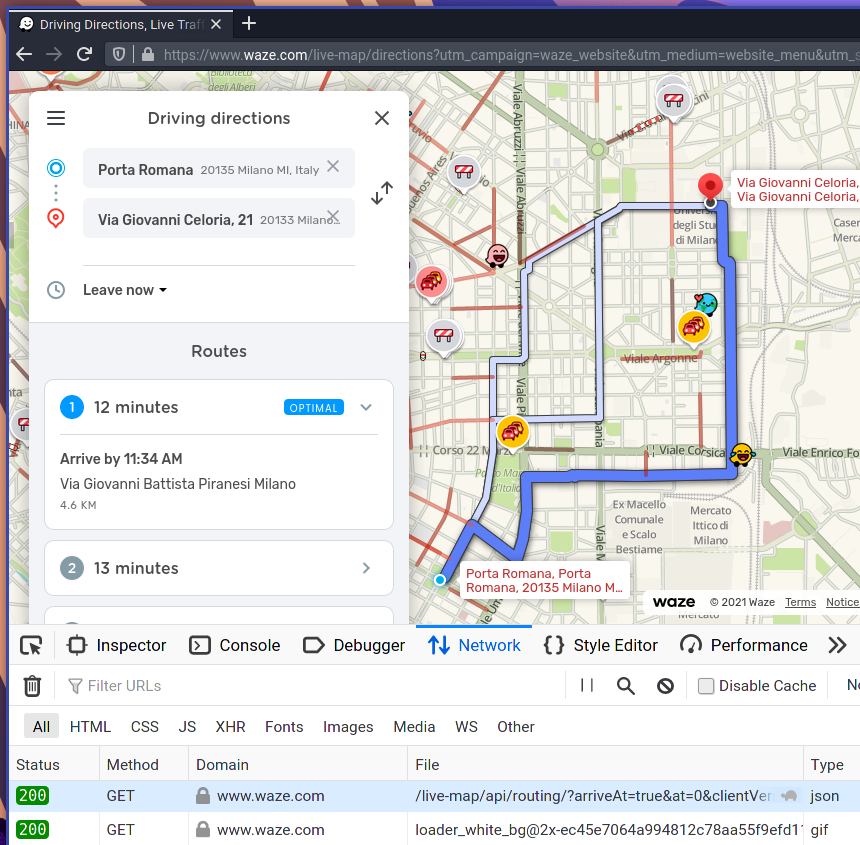
\includegraphics[scale=0.6]{waze_scraping}
	\caption{Console da sviluppatore su Firefox}
	\label{image:1}
\end{figure}
In particolare, la richiesta \url{https://www.waze.com/live-map/routing/?} contiene esattamente il punto di partenza e di arrivo richiesti parametrizzati nell'URL e il risultato restituito è in formato JSON (JavaScript Object Notation)\footnote{\url{https://en.wikipedia.org/wiki/JSON}. Accessed: 20/01/2021}. Per proteggere i loro server da sovraccarichi, Waze risponde a questo URL solamente se si possiede il permesso ricevuto preventivamente tramite un token, ovvero una stringa di caratteri che funge da chiave segreta. Per ottenere questa chiave e raggiungere l'obbiettivo finale di avere delle API per interrogare il servizio, è stato scritto un programma in Go\footnote{\url{https://golang.org/}. Accessed: 20/01/2021} per emulare l'interazione col sito web e ricevere il token necessario per effettuare le richieste successive. Questo processo ha richiesto tempo sia per la codifica dei parametri e sia per la decodifica del risultato stesso e dei risultati intermedi per la richiesta del token. In altre parole, è stato fatto il reverse engineering dell'applicazione web.


\subsection{Lo scraping di Moovit (scartato)}

Inizialmente, prima di usare le API di Here, che offre stime statiche dei tragitti coi mezzi pubblici, si è tanto lo scraping dell'applicazione web di Moovit \url{https://moovitapp.com/} per via della qualità migliore delle stime di percorrenza, basate su dati in tempo reale. Come per lo scraping di Waze, è stato eseguito lo stesso procedimento, guardando tramite la console da sviluppatore del browser le richieste HTTP svolte in background dal sito, studiando tutte le interazioni e decodificando le risposte. Sfortunatamente l'applicazione web è risultata molto più complessa del previsto. Dopo diversi giorni di studio è stato scritto un software per emulare le interazioni della pagina web coi server di Moovit ed è stato affiancato agli altri moduli per risolvere le richieste di tragitto. Le stime di percorrenza relative a Moovit raccolte nella prima settimana di esecuzione del programma sono risultate nulle nell'80\% delle risposte. Visti gli scarsi risultati e vista l'enorme complessità del programma di scraping, si è scelto di optare per le API di Here al costo di perdere precisione nelle stime per i mezzi pubblici.

\subsection{Estratti del codice sorgente degli scraper}

Nei listati seguenti sono riportate le funzioni principali, scritte in Go, addette a interrogare i server dietro ai relativi siti web dei servizi per la tratta richiesta, espressa sotto forma di coordinate geografiche di partenza e arrivo, il cui risultato viene successivamente elaborato e salvato da un altro modulo del programma. Per questioni di leggibilità sono stati omessi i controlli di errore presenti dopo ogni richiesta ed è stata semplificata la sintassi del linguaggio.

\newpage
\subsubsection{Codice dello scraper di Waze}

\begin{lstlisting}[language=Go]
func
GetRoutes(startLat, startLon, endLat, endLon string) Result {
	// Richiesta dei cookies necessari per effettuare
	// le richieste di routing
	cookies := Cookies()
	_       := setCookieConsent()
	
	// Richiesta di tragitti e stime di percorrenza per la
	// tratta desiderata
	return Routes(startLat, startLon, endLat, endLon, cookies)
}
\end{lstlisting}

\subsubsection{Codice dello scraper di Moovit}

\begin{lstlisting}[language=Go]
func
GetRoutes(startLat, startLon, endLat, endLon string) Result {
	// Richiesta del nome canonico della via corrispondente
	// perche' i server non accettano coordinate
	from := LocationName(startLat, startLon)
	to   :=   LocationName(endLat, endLon)
	
	// Richiesta di parametri per fare richieste ai server.
	// Senza di essi i server non accettano altre interazioni
	HTTPHeaders := HeadersNeededForHTTP(from, to)
	cookie      := Cookie(HTTPHeaders)
	_           := SetMagicKey(HTTPHeaders, cookie)
	
	// Richiesta di dati che descrivono la tratta in formato
	// binario (illeggibile)
	fromData    := LocationInfo(from, HTTPHeaders, cookie)
	toData      := LocationInfo(to, HTTPHeaders, cookie)
	
	// Richiesta del token, ovvero la chiave per effettuare
	// le domande ai server. Ne serve una nuova per ogni
	// richiesta
	token := Token(fromData, toData, HTTPHeaders, cookie)
	
	// Richiesta di tragitti e stime di percorrenza per la
	// tratta desiderata
	return Routes(fromData, toData, token, cookie)
}
\end{lstlisting}

\subsection{Stima del percorso per il car sharing}

Avendo a disposizione un servizio di stime di percorrenza per tragitti a piedi e avendo trovato un modo per risolvere quelli in automobile, per il servizio di car sharing Enjoy si è scelto di calcolare una stima sulla base di questi due. Nello specifico, per ogni percorso richiesto viene scaricata la lista aggiornata delle auto libere presenti sul territorio e viene scelta l'auto più vicina calcolando la distanza dal punto di partenza richiesto a ogni auto presente nella lista, scegliendo l'auto con la distanza minima. Una volta trovata vengono richieste e sommate la stima di percorrenza per raggiungere l'auto selezionata a piedi e la stima in automobile dalla posizione di quest'ultima alla destinazione. Sebbene non sia l'approccio migliore, dato che non tiene conto della direzione e del verso di marcia per compiere il viaggio, e quindi rendendo possibile la scelta di un'auto più vicina al punto di partenza ma più lontana dal luogo di destinazione, è risultato il più semplice da programmare e testare.

\section{Scelta tra percorsi random e prefissati}

Si è scelto di usare diverse tratte su cui basare il confronto allo scopo di ricoprire a livello geografico una buona parte del Comune di Milano e di diversificare i confronti in base alle caratteristiche delle tratte, quali lunghezza e punti di partenza e destinazione, per simulare al meglio la posizione di un possibile utente nella mappa. Per rendere automatiche le richieste da inoltrare ai servizi di navigazione è stata scritta una funzione per generare le tratte. Sono stati presi in considerazione tre principali approcci per generarle: hard-coded random; hard-coded di tratte realmente percorse; generazione a random just-in-time.

I primi due approcci sono risultati fin da subito problematici. In primo luogo, la scelta della destinazione avrebbe introdotto bias riguardo al possibile utente del percorso, portando ad analizzare la mobilità solamente dal punto di vista di una determinata categoria, per esempio: selezionare tratte con delle università come punto di arrivo porterebbe ad analizzare la mobilità solamente dal punto di vista degli studenti e dipendenti presso quelle determinate strutture. Altri problemi simili sarebbero sorti nello scegliere la partenza, la lunghezza, la distanza dal centro città e numerosità delle tratte. Seconda problematica molto più rilevante è che, involontariamente, si sarebbero introdotti dei percorsi che avrebbero favorito un mezzo piuttosto che un altro. Nella città di Milano infatti si contano numerosi tratti stradali di questo genere: strade con corsia preferenziale per mezzi pubblici e taxi; strade a singola corsia e con numerosi semafori, quindi più soggetta a incolonnamenti; tangenziali; tratte coperte da passanti ferroviari, che sono più veloci delle metropolitane e con meno fermate. Tale scelta avrebbe portato ad analizzare dati non rappresentativi della città, con conseguenti risultati sbilanciati. Per questi stessi motivi si è deciso di non usare collezioni di dati disponibili da lavori precedenti riguardi servizi di mobilità condivisa, tra cui quelli del car sharing raccolti nel lavoro di Losacco \cite{trentini2017sampling}, ovvero per evitare di analizzare la mobilità dal punto di vista di una sola utenza e per evitare l'inclusione di percorsi strutturalmente più favorevoli a un mezzo rispetto che a un altro.

Usando l'approccio della generazione a random non solo si sarebbero evitati questi problemi, ma i problemi stessi si sarebbero trasformati in analisi da poter eseguire a posteriori, per esempio selezionando da tutte le tratte generate a random quelle che hanno portato nei pressi di un'università, o tratte che in linea d'aria hanno coperto particolari strade favorevoli a determinati mezzi di trasporto. Visti i vantaggi e la flessibilità dell'approccio si è optato per quest'ultimo.

\section{Generatore random dei percorsi}

Prima ancora di scrivere una funzione per generare tratte a random è stata scelta l'area geografica all'interno della quale generarle. Siccome il servizio di car sharing Enjoy non permette di usare la propria flotta al di fuori del Comune di Milano, tale area è stata selezionata come terreno per i confronti, rappresentata sotto forma di rettangolo per questioni di semplicità nella programmazione. Nello specifico sono state scelte le coordinate (45.450562\textdegree, 9.158959\textdegree) e (45.482032\textdegree, 9.206763\textdegree) rispettivamente come vertice in basso a sinistra e in alto a destra del rettangolo rappresentativo dell'area selezionata. In questo modo la generazione di punti a random è stata ridotta alla generazione di coordinate maggiori o uguali della prima e minori o uguali della seconda. Una volta scritta la funzione per la generazione a random delle tratte è stato introdotto un vincolo per simulare dei percorsi scomodi da fare a piedi, ovvero per generare tratte che supererebbero i 20 minuti di camminata per essere coperte, e al tempo stesso che giustificherebbero l'utilizzo dell'automobile. Si è implementato tale vincolo scegliendo di usare 2 km in linea d'aria dal punto di partenza a quello di destinazione come misura minima della lunghezza di una tratta. Un secondo vincolo è stato introdotto per avere una maggiore eterogeneità delle tratte generate a livello geografico. Molte delle linee principali dei mezzi pubblici infatti attraversano il centro storico di Milano e tale area rappresenta più della metà dell'area selezionata dal vincolo precedente. Siccome è stato scelto di ricoprire a livello geografico tutta l'area di Milano, si è programmato il generatore in modo da creare in maniera equidistribuita le seguenti tipologie di tratte: da dentro il centro storico a fuori; da dentro a dentro; da fuori a fuori; da fuori a dentro. Il rettangolo rappresentativo del centro storico è stato disegnato usando le coordinate geografice (45.450562\textdegree, 9.158959\textdegree) e (45.482032\textdegree, 9.206763\textdegree) rispettivamente come vertice in basso a sinistra e in alto a destra.

\section{Timing delle richieste}

Le richieste sono state programmate per essere effettuate dalle 7:00 alle 23:59 di ogni giorno. La scelta di questo intervallo è stata vincolata dall'orario di servizio dei mezzi pubblici ATM in cui viene garantito il pieno regime. Per rispettare i limiti giornalieri delle varie API si è scelto di effettuare 1 richiesta al minuto per un totale di circa 1000 richieste al giorno, dove ogni richiesta rappresenta un tragitto generato a random mandato simultaneamente a ogni servizio di navigazione per ottenere una stima da ognuno di essi.

\section{Codice del programma}

\begin{lstlisting}[language=Go]
func main() {
	var a, b, c coordinate
	
	for {
		a, b = creaTragittoRandom()
		c = enjoy.trovaAutoPiuVicinaOra(a)
		
		risultato := []stime{
			here.stimaTragitto(a, b),
			waze.stimaTragitto(a, b),
			osm.stimaTragitto(a, b, "foot"),
			osm.stimaTragitto(a, b, "bike"),
			osm.stimaTragitto(a, c, "foot") +
				waze.stimaTragitto(c, b)}
		
		save(risultato)
		sleep("1min")
	}
}
\end{lstlisting}